\documentclass[16pt]{beamer}
\usepackage[utf8]{inputenc}
\usepackage[croatian]{babel}
\usepackage{graphicx}
\usepackage{graphicx}
\usepackage{verbatim}
\usepackage{bookmark}
\usepackage{pgfplots}

\graphicspath{ {figures/} }
\usepackage{array}
\usetheme{Warsaw}
\definecolor{mygreen}{rgb}{0.3, 0.73, 0.09}
\setbeamercolor*{palette primary}{use=structure,fg=black,bg=mygreen}
\definecolor{mygreen1}{rgb}{0.0, 0.5, 0.0}
\setbeamercolor*{palette quaternary}{fg=black,bg=mygreen1}
\newcommand\Fontvi{\fontsize{6,5}{7.5}\selectfont}
\pgfplotsset{width=10cm,height=8cm}

\pgfplotsset{every axis/.append style={
                    axis x line=middle,    
                    axis y line=middle,    
                    axis line style={<->,color=blue}, 
                    xlabel={$x$},          
                    ylabel={$y$},          
            }}

\title[IZRADA TABLICA I GRAFIKONA\hspace{20mm} \insertframenumber/\inserttotalframenumber]{IZRADA TABLICA I GRAFIKONA}
\author{Anamaria Vargić \  Jelena Stojković  \  Valentina Ecimović}
\institute{Tehnički fakultet u Rijeci - Računarstvo}
\date{2018}
 
\begin{document}


\frame{\titlepage}
%slajd sa sadrzajem
\begin{frame}

\frametitle{Sadržaj}

\tableofcontents

\end{frame}
\begin{frame}
\frametitle{Lista tabela i slika}


\listoffigures
 
\listoftables
 
\newpage
 
\pagenumbering{arabic}
\end{frame} 

\begin{frame}

\frametitle{Izrada grafikona}

\begin{itemize}
\setlength\itemsep{2em}

\item za vizualiziranje podataka koristimo \textbf{pgfplots} package s kojime dobijemo autogenerirane grafikone
\item osnovna ideja \textbf{pgfplots}-a je da mi unesemo podatke a \textbf{pgfplots} učini ostatak
\item buduci da je \textbf{pgfplots} baziran na \textbf{tikz}-u grafikon se mora nalaziti unutar \textit{tikzpicture} okružja

\end{itemize}

\end{frame}
\begin{frame}[fragile]
\frametitle{Jednostavni grafikoni}

\begin{itemize}
\setlength\itemsep{1em}

\item kako bi uključili \textbf{pgfplots} u dokument u preamblu moramo upisati:
	\begin{verbatim}
		\usepackage{pgfplots}
	\end{verbatim}
\item dodatne postavke za taj paket se mogu upisati u preamblu kao npr:
	\begin{verbatim}
		\pgfplotsset{width=2cm,compat=2.0}
	\end{verbatim}
	width mijenja veličinu svake pgfplot figure na 2 cm,compat određuje koju verziju paketa ćemo koristiti
		
	
\end{itemize}

\end{frame}

\begin{frame}[fragile]

\frametitle{Parametarski grafikon - primjer}
\Fontvi

\begin{verbatim}
\documentclass{article}
\usepackage{pgfplots}
\pgfplotsset{width=15cm,height=15cm} %dimenzije grafa

\pgfplotsset{every axis/.append style={
                    axis x line=middle,    % pozicionira x os u sredinu
                    axis y line=middle,    % pozicionira y os u sredinu
                    axis line style={<->,color=blue}, % stavlja strelice na osi
                    xlabel={$x$},          % označava x-os sa oznakom x
                    ylabel={$y$},          % označava y-os sa oznakom y
            }}

\begin{document}

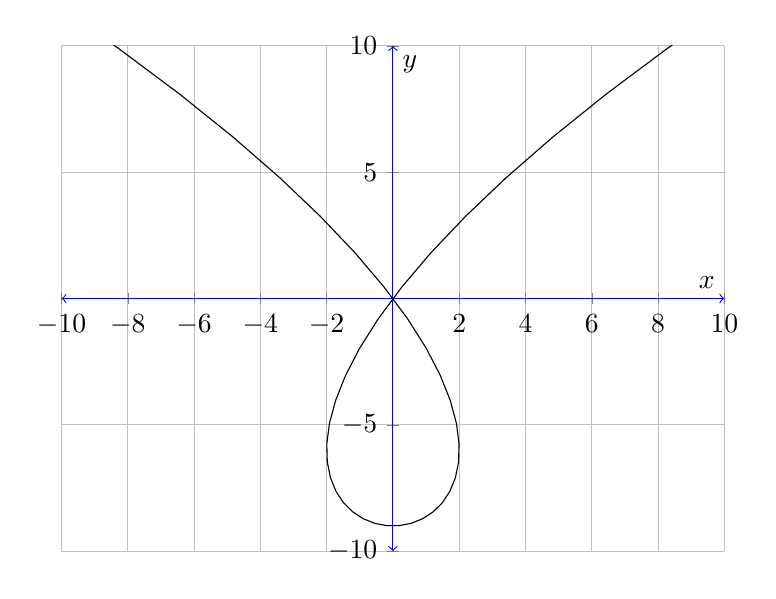
\begin{tikzpicture}  % tikzpicture okružje
    \begin{axis}[
            xmin=-10,xmax=10, % određuje granice x-osi
            ymin=-10,ymax=10, % određuje granice y-osi
            grid=both,
            ]
            \addplot [domain=-3:3,samples=50]({x^3-3*x},{3*x^2-9}); 
    \end{axis}
\end{tikzpicture}
\end{document}
\end{verbatim}



\end{frame}

\begin{frame}[fragile]
\frametitle{Parametarski grafikon - primjer}

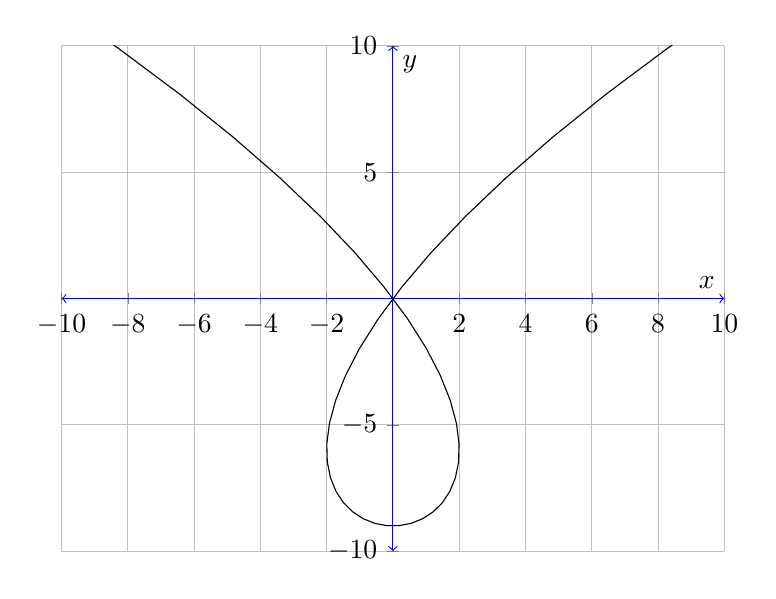
\begin{tikzpicture}
    \begin{axis}[
            xmin=-10,xmax=10,
            ymin=-10,ymax=10,
            grid=both,
            ]
            \addplot [domain=-3:3,samples=50]({x^3-3*x},{3*x^2-9}); 
    \end{axis}
\end{tikzpicture}
\end{frame}

\end{document}


 
 

